\documentclass[a4paper,12pt]{article}
\usepackage[magyar]{babel}
\usepackage{times}
\usepackage[utf8x]{inputenc}
\usepackage[T1]{fontenc}
\usepackage{lmodern}
\usepackage[intlimits,sumlimits]{amsmath}
\usepackage{amssymb}
\usepackage{graphicx}
\usepackage{hyperref}
% listings begin
\usepackage{color}
\usepackage{xcolor}
\usepackage{listings}
\lstset{literate=%
{Ö}{{\"O}}1
{Ä}{{\"A}}1
{Ü}{{\"U}}1
{ß}{{\ss}}2
{ü}{{\"u}}1
{ä}{{\"a}}1
{ö}{{\"o}}1
{é}{{\'e}}1
{ő}{{\"o}}1
{á}{{\'a}}1
{ó}{{\'o}}1
{í}{{\'i}}1
{ú}{{\'u}}1
{ű}{{\"u}}1
}
\usepackage{caption}
\DeclareCaptionFont{white}{\color{white}}
\DeclareCaptionFormat{listing}{\colorbox{gray}{\parbox{\textwidth}{#1#2#3}}}
\captionsetup[lstlisting]{format=listing,labelfont=white,textfont=white}
% listings end
%opening
\author{MusicSeeker}
\title{Szoftverarchitektúrák NagyHF}
\date{\today}
\begin{document}
%%%%%%%%%%%%%%%%%%%Címoldal%%%%%%%%%%%%%%%%%%%%%%
\begin{titlepage}
\begin{center}
\vspace*{\fill}
\hrulefill\\[0.5cm]
  \textsc{\LARGE Követelményspecifikáció}\\[0.5cm] 
  \textsc{\Large Melyik zeneszolgáltatást válasszam? }\\[0.2cm]
  \textsc{\large Szoftverarchitektúrák tárgy házi feladat}\\[0.5cm]
\hrule
 \end{center}
 \vspace{3cm}
\begin{minipage}{0.4\textwidth}
\begin{flushleft} \large
Készítette:\\[0.2cm]
\textsc{Fekete} Norbert Zoltán\\[0.2cm]
CO0DA1\\
feno26@gmail.com
\end{flushleft}
\end{minipage}
\begin{minipage}{0.6\textwidth}
\begin{flushleft} \large
\vspace{0.82cm}
\textsc{Unicsovics} Milán György\\[0.2cm]
M9GNTV\\
u.milan@gmail.com
\end{flushleft}
\end{minipage}
\vspace*{\fill}
\end{titlepage}
%%%%%%%%%%%%%%%%%%%Szöveg%%%%%%%%%%%%%%%%%%%%%%

\section{Feladatkiírás}
\label{sec:feladatkiiras}

A felhasználó eszközein (asztali PC vagy mobileszköz) tárolt zenéi alapján a rendszer megadja, hogy melyik zeneszolgáltatás katalógusában (Spotify, Deezer, Google Music,iTunes) található meg a legtöbb a tárolt zenék közül. Ehhez a különböző zeneszolgáltatások API-ját használja fel.

% section feladatkiiras (end)

\section{A fejlesztői csapat}
\label{sec:afejlesztoicsapat}

A csapat tagjai:

\begin{table}[htb]
\begin{center}
\begin{tabular}{|l|l|l|}
\hline
\textbf{Csapattag neve} & \textbf{Neptun-kód} & \textbf{E-mail cím} \\ \hline
Fekete Norbert Zoltán & CO0DA1 & feno26@gmail.com \\ \hline
Unicsovics Milán György & M9GNTV & u.milan@gmail.com \\ \hline
\end{tabular}
\end{center}
\label{tab:acsapattagjai}
\caption{A csapat tagjai}
\end{table}

A csapatban dedikált szerepek kiosztását a csapat kis mérete miatt nem tartottuk fontosnak.

% section afejlesztoicsapat (end)

\section{Részletes feladatleírás}
\label{sec:reszletesfeladatkiiras}

A projekt során célunk egy olyan alkalmazás készítése, amely segít a felhasználónak eligazodni a manapság egyre inkább elterjedő internetes zenei szolgáltatások világában. Ezt a felhasználó meglévő zenei gyűjteményének letapogatásával, majd annak a felhő alapú szolgáltatók készleteivel történő összevetésével éri el.

Az alapvető keresési egység a zenei album lesz. Az elemzési folyamat végeztével a felhasználó egy statisztikát kap, melyből kiolvashatja, mely zeneszolgáltatás gyűjteményével a legnagyobb az átfedés - vagyis mely szolgáltatónál találhat a legkönnyebben a saját stílusának megfelelő zenéket.

Emellett egyszerű, kulcsszavas keresésre is lesz lehetőség (meglévő zenefájlok nélküli kereséshez), amivel kényelmesen lehet majd egyszerre több szolgáltató készletét is lekérdezni.

A program első megközelítésben a \textit{Deezer}, a \textit{Spotify}, az \textit{iTunes} és a \textit{Last.Fm} szolgáltatásait fogja támogatni, de célunk egy általános architektúra kialakítása, mely később könnyedén bővíthető további szolgáltatásokkal (pl.: \textit{Google Play Music}).

% section reszletesfeladatkiiras (end)

\section{Technikai paraméterek}
\label{sec:technikaiparameterek}

A definiált alkalmazást Python platformra készítjük el annak érdekében, hogy több operációs rendszeren (Windows, Linux, Mac OS) is lehessen használni.  Szükség lesz ezen kívül néhány Python-os könyvtárhoz, ezeket a Python csomagkezelőjével (\textit{pip}) egyszerűen lehet majd telepíteni.

A program felhasználói felületét \href{http://python-gtk-3-tutorial.readthedocs.org/en/latest/}{Python GTK+ 3} segítségével fogjuk elkészíteni, a GUI-t magát deklaratív módon \href{https://glade.gnome.org/}{Glade} segítségével állítjuk elő.

Külső függőségeink közé tartoznak a zeneszolgáltatások API-jai is:

\begin{itemize}
	\item \href{https://developer.spotify.com/web-api/}{Spotify}
    \item \href{http://developers.deezer.com/api/}{Deezer}
    \item \href{https://www.apple.com/itunes/affiliates/resources/documentation/itunes-store-web-service-search-api.html}{iTunes}
    \item \href{http://www.last.fm/api}{Last.fm}
    \item \href{http://unofficial-google-music-api.readthedocs.org/en/latest/}{(Google Music)}
\end{itemize}

A fent felsorolt külső függőségek sebességének függvényében, lehet, hogy szükség lesz valamilyen szerver oldali komponens fejlesztésére is, amely egy fajta cache-ként szolgálva gyorsíthatja a program működését. A szerver elérhetősége viszont a program funkcionalitását nem befolyásolja.

% section technikaiparameterek (end)

\section{Szótár}
\label{sec:szotar}

% section szotar (end)

\begin{description}
    \item[Zeneszolgáltatás] Kereskedelmi streamelő alkalmazás, melyben a fehasználó zenéket hallgathat illetve vásárolhat.
    \item[Zeneállomány] A zeneszolgáltatás vagy a felhasználó által birtokolt zenealbumok összessége.
    \item[Zenei katalógus] A zeneszolgáltatás kereshető zeneállománya.
    \item[Kiértékelési statisztika] A felhasználó által megtekinthető grafikus szemléltető eszköz, mely arra szolgál, hogy az egyes zeneszolgáltatásoknál, mely zenealbumok érhetőek el.
    \item[Zeneállomány felderítése] A felhasználó által megadott helyen az elérhető zenealbumok és azok adatainak összegyűjtése.
    \item[Keresés zenékre] Minden támogatott zeneszolgáltató átvizsgálása, hogy egy bizonyos zenealbum elérhető-e az adott platformon.
\end{description}

\section{Essential use-case-ek}
\label{sec:usecaseek}

\subsection{Use-case diagram}
\label{sub:ucdiagram}

\begin{figure}[htp]
\centering
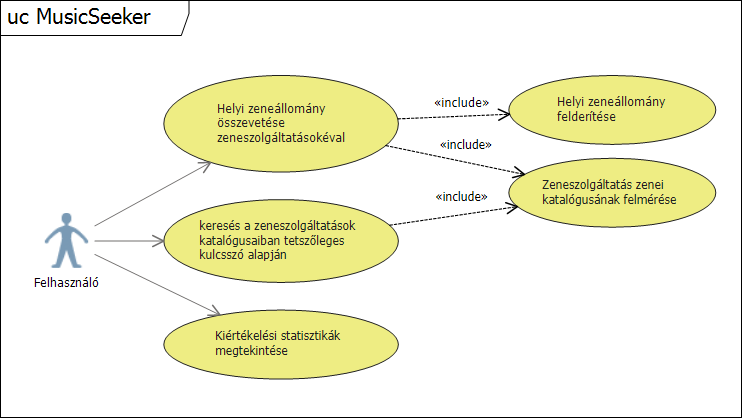
\includegraphics[scale=0.8]{img/01_UseCases.png}
\caption{A MusicSeeker use case diagramja}
\label{fig:01_UseCases}
\end{figure}


% subsection ucdiagram (end)

% section usecaseek (end)


\end{document}
